\section{Podejście wariacyjne - metoda Rayleigha-Ritza}

%%%%%%%%%%%%%%%% 
	
	\begin{frame}{Podejście wariacyjne - metoda Rayleigha-Ritza}
		Przypomnienie:
		
		\begin{block}{Rachunek wariacyjny}
			Metody wyznaczania funkcji $y(x)$, dla której dany funkcjonał przyjmuje wartość ekstremalną
		\end{block}
		
		\begin{itemize}
			\item $F(x,y,y')$ - funkcja klasy $C^2[a,b]$
					
			\item $\Omega_0$ - zbiór funkcji $y = y(x)$, klasy $C^1[a,b]$:
					
			\item $y(x_1) = y_1$ ; $y(x_2) = y_2$ ; $y_1, y_2$ - dane liczby
		\end{itemize}
		
	\end{frame}

%%%%%%%%%%%%%%%% 
	
	\begin{frame}{Funkcjonał}
		\begin{block}{Funkcjonał:}
			$I[y] = \int_a^b F(x,y,y') dx$
		\end{block}		
		\begin{columns}
			\column{0.38\linewidth} 
				\begin{figure}
					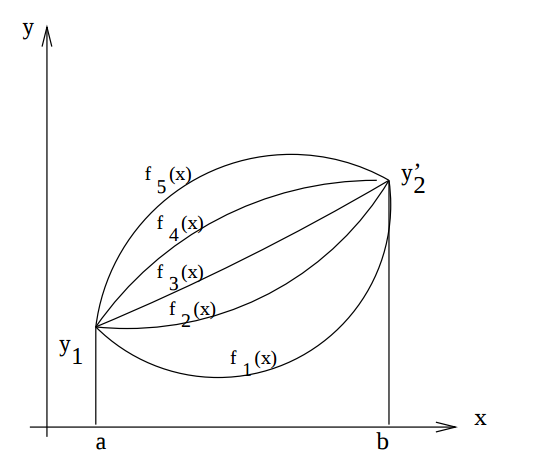
\includegraphics[width=1.2\textwidth]{img/19/functional}
				\end{figure}
			\column{0.58\linewidth} 
				Spośród wszystkich $y_i(x)$ należy wybrać tę, która ekstremalizuje $I[y]$.
					
				Wartość $I[y]$ zależy od funkcji, a nie od liczby $\rightarrow$ stąd nazwa: \textbf{funkcjonał}
		\end{columns}	
		
		
		
	\end{frame}
	
%%%%%%%%%%%%%%%% 

	\begin{frame}{Równanie Eulera-Lagrange'a}
		Warunkiem koniecznym istnienia ekstremum $I[y]$ jest spełnienie przez $F(x,y,y')$ następującego równania:
		
		\begin{block}{Równanie Eulera-Lagrange'a}
			$$
			F_y - \frac{d}{dx} F_{y'} = 0
			$$
			
			$F_y , F_{y'}$ - odpowiednie pochodne cząstkowe
		\end{block}
		
		
		
	\end{frame}

%%%%%%%%%%%%%%%% 

	\begin{frame}{Znalezienie funkcji bez rozwiązywania równania}
	
		Łatwo sprawdzić, że:
		%nie przypadkiem \varphi_x ?
		$$
		\varphi_{xx}(x) + \varphi(x) = \alpha
		$$
				
		jest równaniem Eulera-Lagrange'a funkcjonału:
				
		$$
		I[\varphi] = \int_0^{\frac{\pi}{2}} \underbrace{[\frac{1}{2}(\varphi_x)^2 - \frac{1}{2}\varphi^2 + \alpha \varphi]}_{F(x,\varphi, \varphi_x)} dx
		$$
		Zamiast rozwiązywać równanie różniczkowe, szukamy funkcji:
		$$
		\begin{cases}
			\varphi(x) \in C^2[0, \frac{\pi}{2}] \\
			\varphi(0) = \varphi(\frac{\pi}{2}) = 1 \\
			\text{aproksymującej min } I[\varphi]
		\end{cases}
		$$		
	\end{frame}
	
%%%%%%%%%%%%%%%% 

	\begin{frame}{Znalezienie funkcji bez rozwiązywania równania - układ współrzędnych}
		Niech: $\varphi_0(x), \varphi_1(x), ... , \varphi_i(x), ... \leftarrow$ dany:
			\begin{itemize}
				\item ciąg liniowo niezależnych funkcji
				\item tworzących na odcinku $[0, \frac{\pi}{2}]$ ukłąd zupełny
				\item $\varphi_i \in C^2 [0, \frac{\pi}{2}]$
			\end{itemize}
			
			Ciąg $\{\varphi_i\}$ nosi nazwę układu funkcji współrzędnych lub układu współrzędnych
			
			$$
			U_n(x) = \sum_{i=0}^{N+1} a_i \varphi_i \leftarrow \text{ aproksymacja min}
			$$
			
			$a_0, a_{N+1} \leftarrow$ uzyskujemy z warunków logicznych
			
			$a_i, i = 1,2, ... , N$ - z warunku minimum funkcjonału $I[U_N]$
	
	\end{frame}

%%%%%%%%%%%%%%%% 
	
	\begin{frame}{Znalezienie funkcji bez rozwiązywania równania - postać jawna}
		$$
		\frac{\partial I[U_N]}{\partial a_j} = 0, j = 1,2, ... , N
		$$
					
		Jawna postać - po podstawieniu $U_N(x)$ do $I$
					
		W rezultacie - do rozwiązania układu N równań liniowych o N niewiadomych $a_i$
					
	\end{frame}

%%%%%%%%%%%%%%%% 

	\begin{frame}{Uwagi}
		\begin{itemize}
			\item takie $\varphi_i(x)$ by szybko uzyskać zbieżność aproksymacji $U_N$ (tj. małe N)
			\item proste całkowania w I
		\end{itemize}
		
		$\rightarrow$ sprzeczne wymagania \\
		$\rightarrow$ niebezpieczeństwo, że macierz współczynników będzie źle uwarunkowana - np. dla:
		$$
		\varphi_i = a_i \cdot x^i
		$$
	
	\end{frame}

%%%%%%%%%%%%%%%% 
	
	\begin{frame}{Uwagi - układ współrzędnych}
		Układ współrzędnych:
		\begin{itemize}
			\item wielomiany ortogonalne
			\item funkcje trygonometryczne
		\end{itemize}
		
		
		Pod całką nie ma $\varphi_{xx} \rightarrow$ dla istnienia $I[\varphi]$ wystarczy, by $\varphi_x$ była odcinkami ciągła
		\begin{itemize}
			\item W jakiej klasie funkcji szukać przybliżenia?	
			\item Kiedy istnieje minimum funkcjonału?
		\end{itemize}	
		
		Czy zawsze dla RR istnieje odpowiedni funkcjonał?
		
		Trudności z uwzględnieniem złożonych warunków brzegowych lub początkowych
	\end{frame}


